\chapter{Einleitung}
%
%
%
%
%
%
Jedes Jahr wird weltweit das Leben von etwa 1,3 Millionen Menschen durch einen Verkehrsunfall beendet. Zwischen 20 und 50 Millionen weitere Menschen erleiden nicht-tödliche Verletzungen, wobei viele infolge ihrer Verletzung eine Behinderung erleben müssen. Verkehrsunfälle verursachen erhebliche wirtschaftliche Verluste für Einzelpersonen, ihre Familien und Nationen insgesamt. Diese Verluste ergeben sich aus den Behandlungskosten sowie aus Produktivitätsverlusten für diejenigen, die durch ihre Verletzungen getötet oder behindert wurden, und für Familienmitglieder, die sich von der Arbeit oder Schule freinehmen müssen, um sich um die Verletzten zu kümmern. Straßenverkehrsunfälle kosten die meisten Länder 3\% ihres Bruttoinlandsprodukts. Verletzungen im Straßenverkehr sind die häufigste Todesursache für Kinder und junge Erwachsene im Alter von 5 bis 29 Jahren.\citep{healthorganization2022}

Motorradfahren findet in Deutschland immer mehr Zuwachs.  Rund 3,8 Millionen zweirädrige Kraftfahrzeuge waren am 1. Januar 2012 in Deutschland zugelassen. Dies entspricht 7,26 \% aller zugelassener Kraftfahrzeuge in Deutschland \citep{Haedrich2012}.

Motorradfahrer stellen im Straßenverkehr eine besonders gefährdete Gruppe an Verkehrsteilnehmern dar. Die NHTSA schätzt, dass Motorradfahrer im Jahr 2018 etwa 27-mal häufiger bei Verkehrsunfällen in den USA ums Leben kamen als Insassen von PKWs\citep{NHTSA}.

Verzögerungen bei der Erkennung und Behandlung der an einem Verkehrsunfall beteiligten Personen erhöhen die Schwere der Verletzungen. Die Versorgung von Verletzungen nach einem Unfall ist äußerst zeitkritisch. Verzögerungen von Minuten können über Leben und Tod entscheiden. Die Verbesserung der Versorgung nach einem Unfall erfordert die Sicherstellung des Zugangs zu rechtzeitiger präklinischer Versorgung und die Verbesserung der Qualität sowohl der präklinischen als auch der stationären Versorgung.\citep{healthorganization2022}

Da die Reaktionszeit der Rettung eine besonders große Rolle dabei spielt, Leben zu retten, ist eine automatische Unfallerkennung von großen Bedeutung.

Bosch hat ein neues Notrufsystem namens "'Help Connect"' auf den Markt gebracht, das automatisch Hilfe rufen kann, wenn es Unfälle auf Motorrädern erkennt.
Der Dienst nutzt einen Unfallerkennungsalgorithmus, um festzustellen, ob ein Motorrad wirklich in einen Unfall verwickelt oder nur umgestürzt ist.
Wenn "'Help Connect"' entscheidet, dass ein Motorrad in einem Unfall war, übermittelt es Informationen über die Unfallstelle und den Fahrer wie z.B. der aktuelle Standort, der Schweregrad des Aufpralls und die optional hinterlegte Gesundheitsdaten an das Bosch Service Center.
Im Call-Center versuchen speziell geschulte Agenten, den Fahrer zu erreichen. Wenn der zu erreichten Fahrer nicht reagiert und die Sensoren einen schweren Unfall erkannt haben, wenden sie sich mit allen Informationen an die lokale Rettungsdienste, damit sie der Person so schnell wie möglich helfen können.\Citep{Gibbons2021}\Citep{Moon2020}\Citep{BoschPresse2021}

Die \autoref{fig:HelpConnect} fasst die Ablaufschritte im Fall einer Unfallerkennung zusammen. Nachdem ein Motorradunfall durch das Smartphone erkannt wird, wird eine Benachrichtigung an Bosch Call-Center mit der Unfallschwere. Der Agent versucht den Fahrer telefonisch zu erreichen, der den Unfall bestätigt oder absagt. Wenn die Person Hilfe benötigt, gibt der Agent die notwendige Informationen an die lokale Rettungsdienste weiter.

Diese Arbeit beschäftigt sich mit der Weiterentwicklung des Unfallerkennungsalgorithmus, damit dieser auch im Taschenmodus verwendbar und funktionsfähig bleibt. Darunter fällt die Ermittlung der potenziellen Verhaltensunterschiede des Algorithmus' zwischen dem originalen Modus (Am Lenker) und dem Taschenmodus. Anpassungsideen werden vorgeschlagen und bei bestimmten Szenarien entwickelt und verifiziert.

\begin{figure}
	\centering
	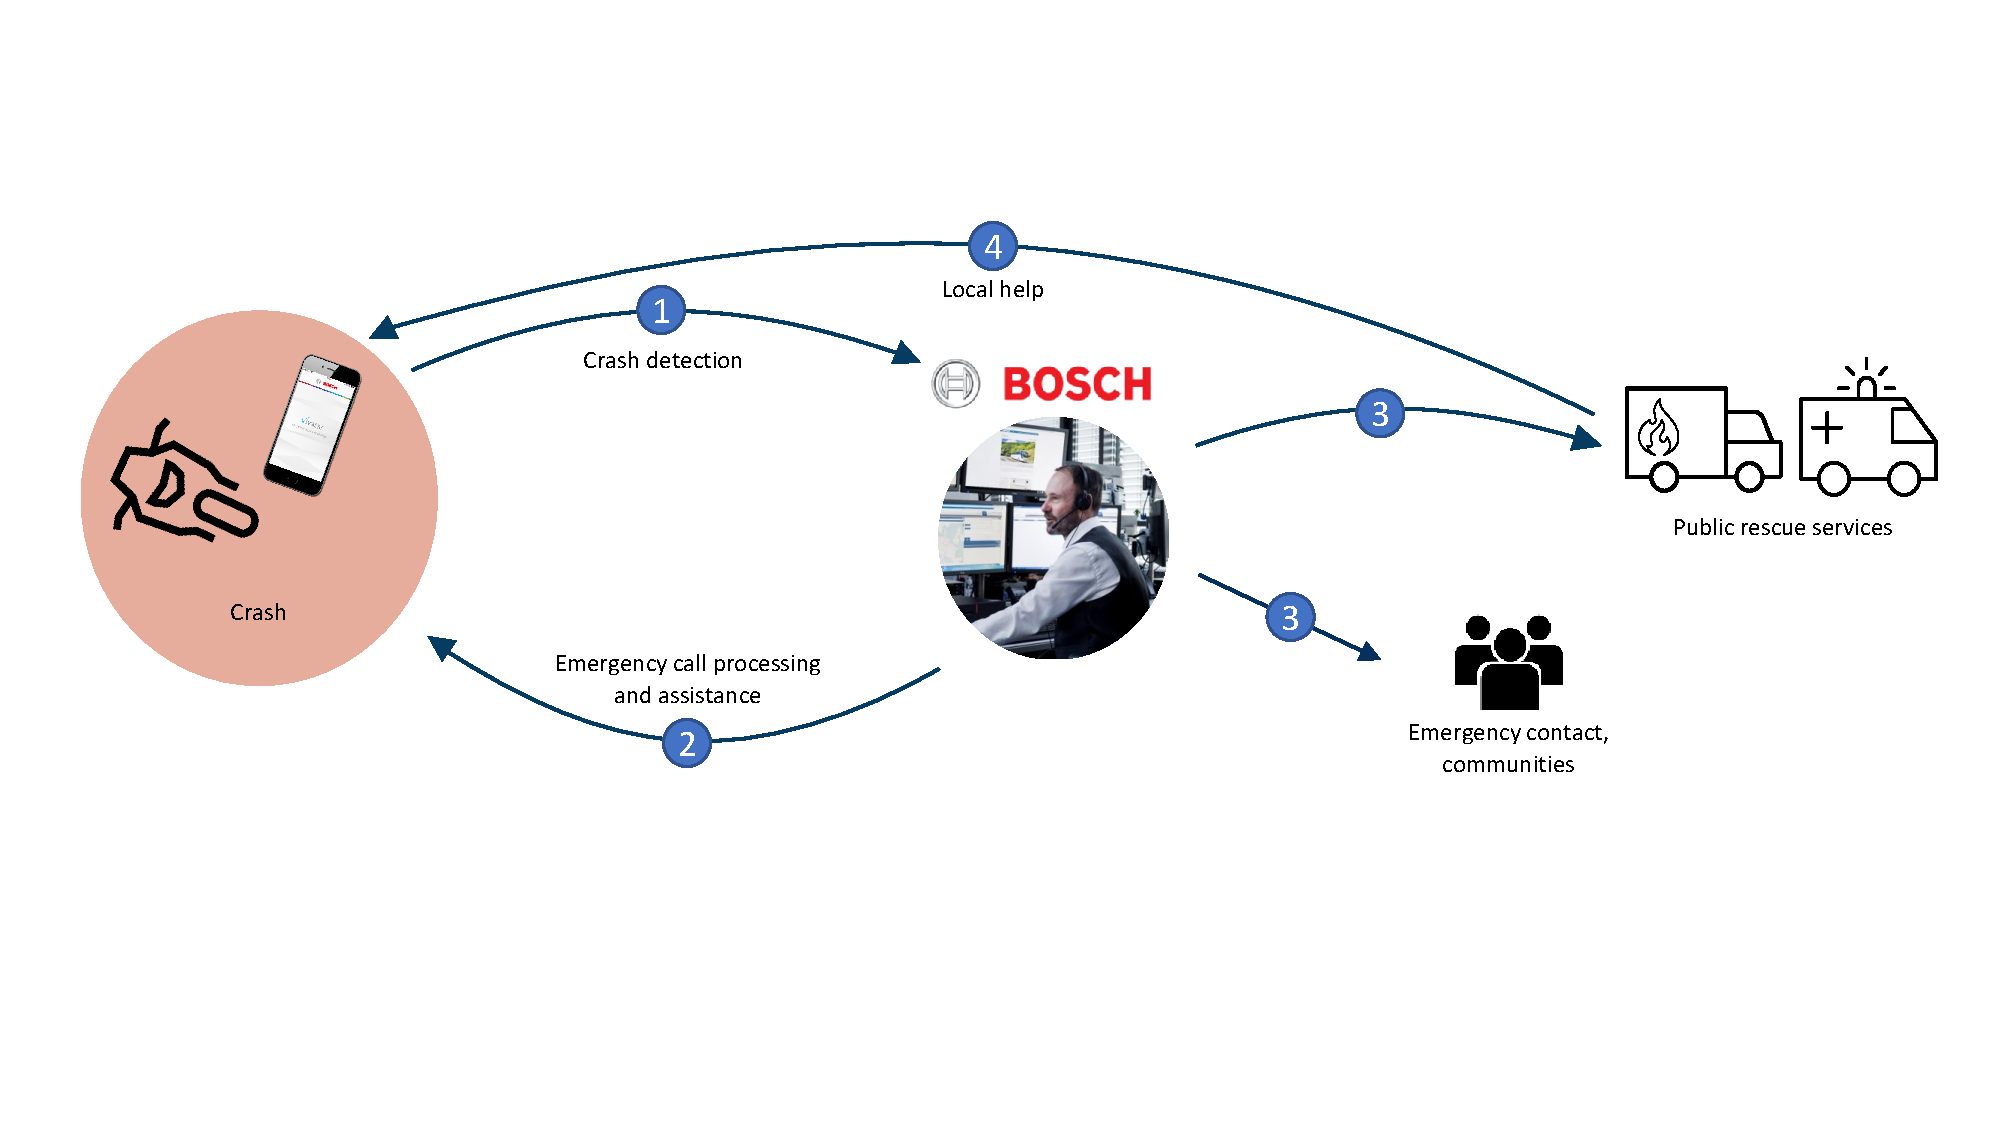
\includegraphics[width=\linewidth]{Bilder/HelpConnect.pdf}
	\caption{Umgang der Funktion '"Help Connect"' im Fall eines Motorradunfalls}
	\label{fig:HelpConnect}
\end{figure}


%Diese Arbeit beschäftigt sich mit der Weiterentwicklung eines Unfallerkennungsalgorithmus mittels Smartphone. \\
%- Pocket-Mode\\
%- Edgecases\\
%- Mögliche Maßnahmen\\
%- 











